\documentclass[en,mtpro2]{elegantpaper}

\title{Notes: Double/Debiased Machine Learning}
\author{Ziyang Gong}

\usepackage{subcaption}

\begin{document}

\maketitle

\section{Intutation}

Consider the partical linear regression model
\begin{equation}
    \begin{aligned}
        Y_{i}=D_{i}\theta+g(\mathbf{X}_{i})+U_{i}, & \quad E\left(U_{i}\mid\mathbf{X}_{i},D_{i}\right)=0 \\
        D_{i}=m(\mathbf{X}_{i})+V_{i},             & \quad E\left(V_{i}\mid\mathbf{X}_{i}\right)=0
    \end{aligned}
\end{equation}
where $\mathbf{X}_{i}\in\mathbb{R}^{p}$, $i=1,2,\ldots,n$. Suppose
\begin{equation}
    \begin{aligned}
        m(\mathbf{X}_{i})= & \gamma_{1}x_{i,1}+\gamma_{2}x_{i,2}+\gamma_{3}x_{i,3}+U_{i} \\
        g(\mathbf{X}_{i})= & \beta_{1}x_{i,1}+\beta_{2}x_{i,2}+\beta_{3}x_{i,3}+V_{i}
    \end{aligned}
\end{equation}
and
\begin{equation*}
    n=1000,\quad p=200,\quad\boldsymbol{\gamma}=\left(3,2,1\right)^{\prime},\quad\boldsymbol{\beta}=\left(1,2,3\right)^{\prime}
\end{equation*}

\subsection{Regularization Bias}

\begin{enumerate}
    \item Non Orthogonal: Suppose $\hat{g}$ are estimated using the auxiliary samples indexed by $\mathrm{I}^{c}$, thus
          \begin{equation}
              \check{\theta}=\left(\frac{1}{n}\sum_{i\in\mathrm{I}}D_{i}^{2}\right)^{-1}\frac{1}{n}\sum_{i\in\mathrm{I}}D_{i}\left(Y_{i}-\hat{g}\left(X_{i}\right)\right)
          \end{equation}
    \item Orthogonal:  Suppose $\hat{g}$ and $\hat{m}$ are estimated using the auxiliary samples indexed by $\mathrm{I}^{c}$, thus
          \begin{equation}
              \check{\theta}=\left(\frac{1}{n}\sum_{i\in\mathrm{I}}\widehat{V}_{i}D_{i}\right)^{-1}\frac{1}{n}\sum_{i\in\mathrm{I}}\hat{V}_{i}\left(Y_{i}-\hat{g}\left(X_{i}\right)\right)
          \end{equation}
          where $\hat{V}=D-\hat{m}(\mathbf{X})$.
\end{enumerate}

\begin{figure}[htpb]
    \centering
    \begin{subfigure}{.45\textwidth}
        \centering
        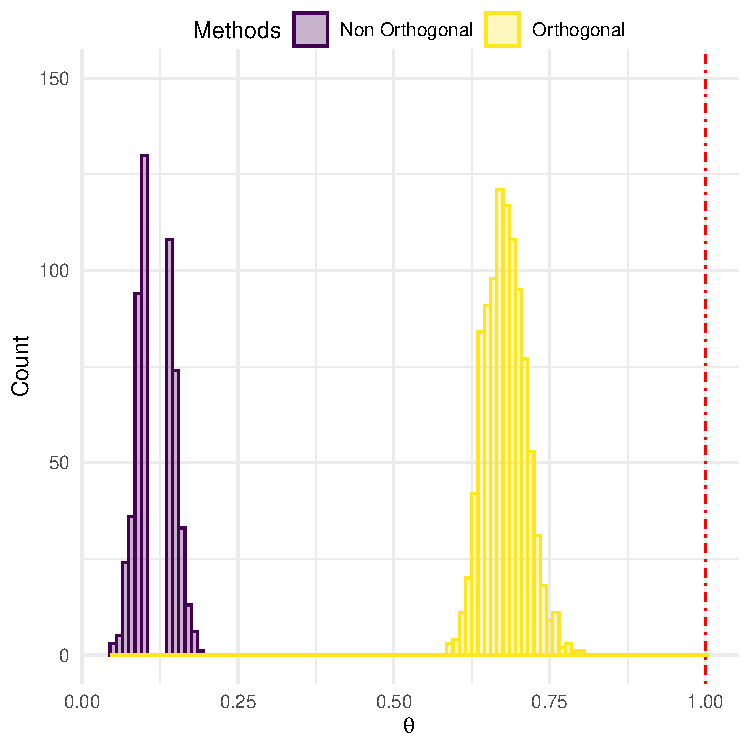
\includegraphics[width=\linewidth]{figures/intution-non-orthogonal-vs-orthogonal-lasso.pdf}
        \caption{LASSO}
    \end{subfigure}
    \begin{subfigure}{.45\textwidth}
        \centering
        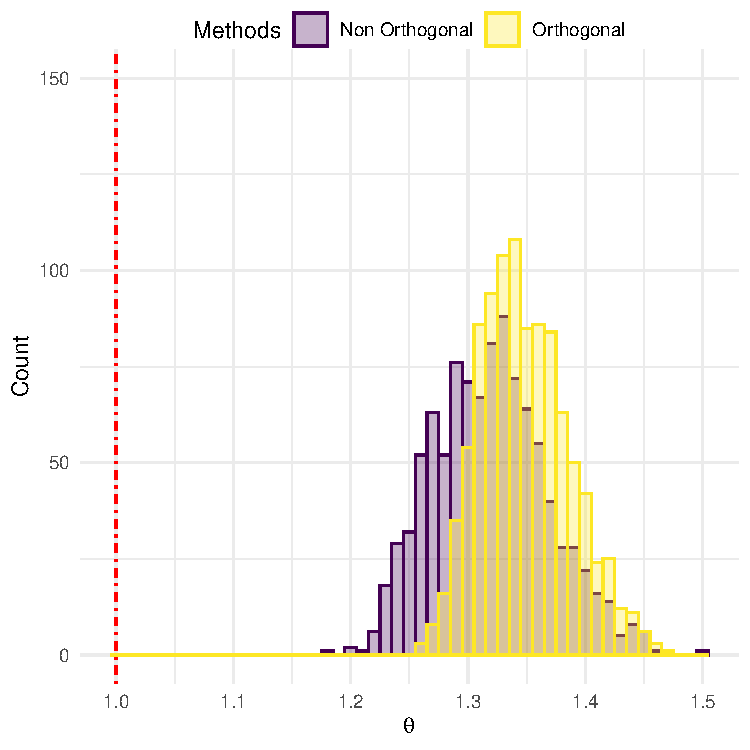
\includegraphics[width=\linewidth]{figures/intution-non-orthogonal-vs-orthogonal-rf.pdf}
        \caption{Random Forest}
    \end{subfigure}
    \caption{Bias Raised by Regularization of Machine Learning}
\end{figure}

\subsection{Overfitting Bias}

\begin{figure}[htpb]
    \centering
    \begin{subfigure}{.45\textwidth}
        \centering
        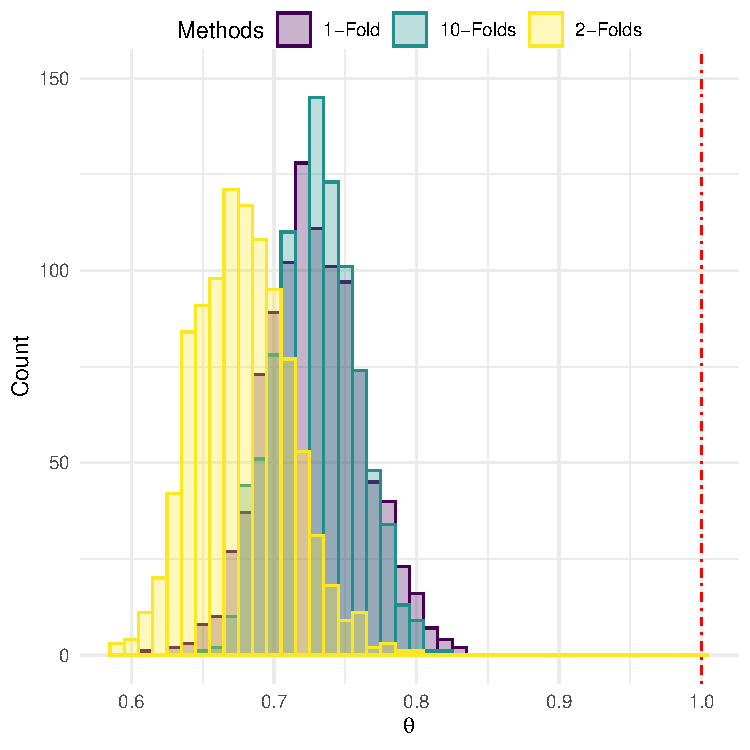
\includegraphics[width=\linewidth]{figures/intution-full-sample-vs-split-sample-lasso.pdf}
        \caption{LASSO}
    \end{subfigure}
    \begin{subfigure}{.45\textwidth}
        \centering
        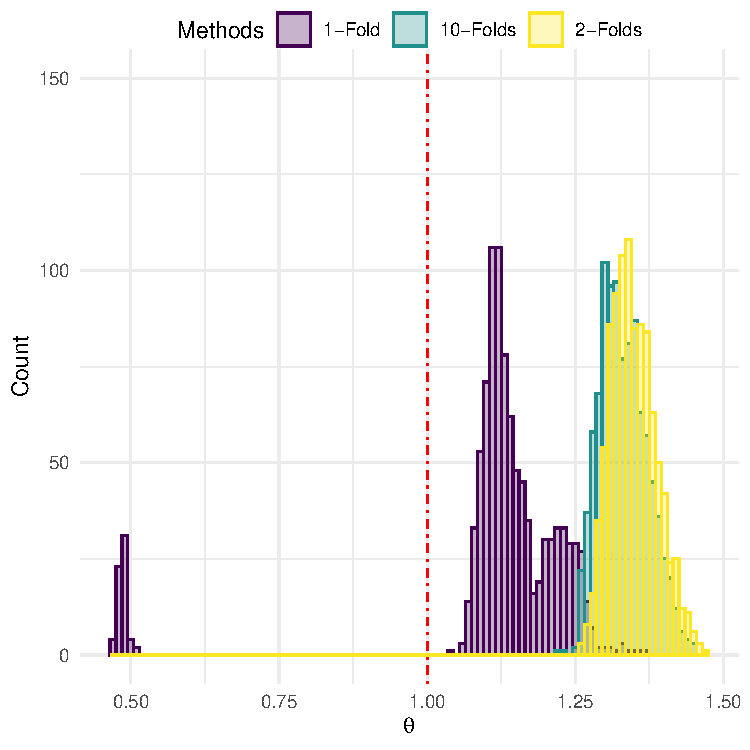
\includegraphics[width=\linewidth]{figures/intution-full-sample-vs-split-sample-rf.pdf}
        \caption{Random Forest}
    \end{subfigure}
    \caption{Bias Raised by Overfitting of Machine Learning}
\end{figure}

\subsection{Score Functions}

\begin{definition}[Neymaxn Orthogonal Score Function]

\end{definition}

\begin{remark}
    Suppose the score function is the linearity function of in the parameter $\theta$, that,
    \begin{equation}
        \psi\left(\mathbf{W};\theta,\boldsymbol{\eta}\right)=\psi_{a}\left(\mathbf{W};\boldsymbol{\eta}\right)\theta+\psi_{b}\left(\mathbf{W};\boldsymbol{\eta}\right)
    \end{equation}
    Hence the estimator can be written as
    \begin{equation}
        \check{\theta}=-\frac{\mathbb{E}_{N}\left[\psi_{b}\left(\mathbf{W};\boldsymbol{\eta}\right)\right]}{\mathbb{E}_{N}\left[\psi_{a}\left(\mathbf{W};\boldsymbol{\eta}\right)\right]}
    \end{equation}
\end{remark}

\begin{enumerate}
    \item IV-type: The score function of IV-type is
          \begin{equation}
              \psi\left(\mathbf{W};\theta,\boldsymbol{\eta}\right):=\left[Y-D\theta-g(\mathbf{X})\right]\left[D-m(\mathbf{X})\right]
          \end{equation}
          where $\boldsymbol{\eta}=(g,m)$. Suppose $\hat{g}$ and $\hat{m}$ are estimated using the auxiliary samples indexed by $\mathrm{I}^{c}$, Thus
          \begin{equation}
              \check{\theta}=\left(\frac{1}{n}\sum_{i\in\mathrm{I}}\widehat{V}_{i}D_{i}\right)^{-1}\frac{1}{n}\sum_{i\in\mathrm{I}}\hat{V}_{i}\left(Y_{i}-\hat{g}\left(X_{i}\right)\right)
          \end{equation}
          where $\hat{V}=D-\hat{m}(\mathbf{X})$.
    \item Partialling-Out: The score function of partialling-out is
          \begin{equation}
              \psi\left(\mathbf{W};\theta,\boldsymbol{\eta}\right):=\left[Y-\ell\left(\mathbf{X})-\theta\left(D-m(\mathbf{X}\right)\right)\right]\left[D-m(\mathbf{X})\right]
          \end{equation}
          where $\boldsymbol{\eta}=(\ell,m)$. Suppose $\hat{\ell}$ and $\hat{m}$ are estimated using the auxiliary samples indexed by $\mathrm{I}^{c}$, Thus
          \begin{equation}
              \check{\theta}=\left(\frac{1}{n}\sum_{i\in\mathrm{I}}\widehat{V}_{i}^{2}\right)^{-1}\frac{1}{n}\sum_{i\in\mathrm{I}}\hat{V}_{i}\left(Y_{i}-\hat{\ell}\left(X_{i}\right)\right)
          \end{equation}
          where $\hat{V}=D-\hat{m}(\mathbf{X})$.
\end{enumerate}

\begin{figure}[htpb]
    \centering
    \begin{subfigure}{.45\textwidth}
        \centering
        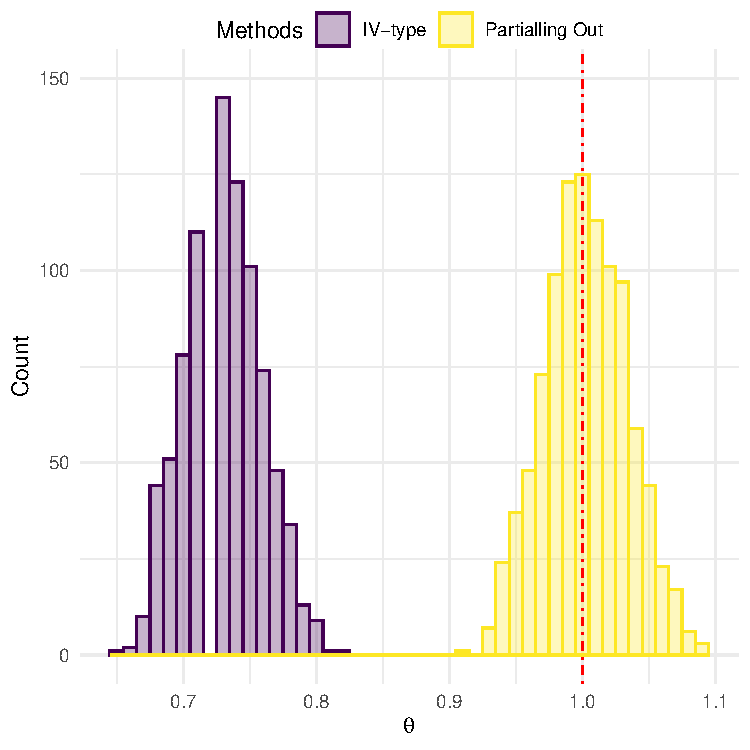
\includegraphics[width=\linewidth]{figures/intution-iv-type-vs-partialling-out-lasso.pdf}
        \caption{LASSO}
    \end{subfigure}
    \begin{subfigure}{.45\textwidth}
        \centering
        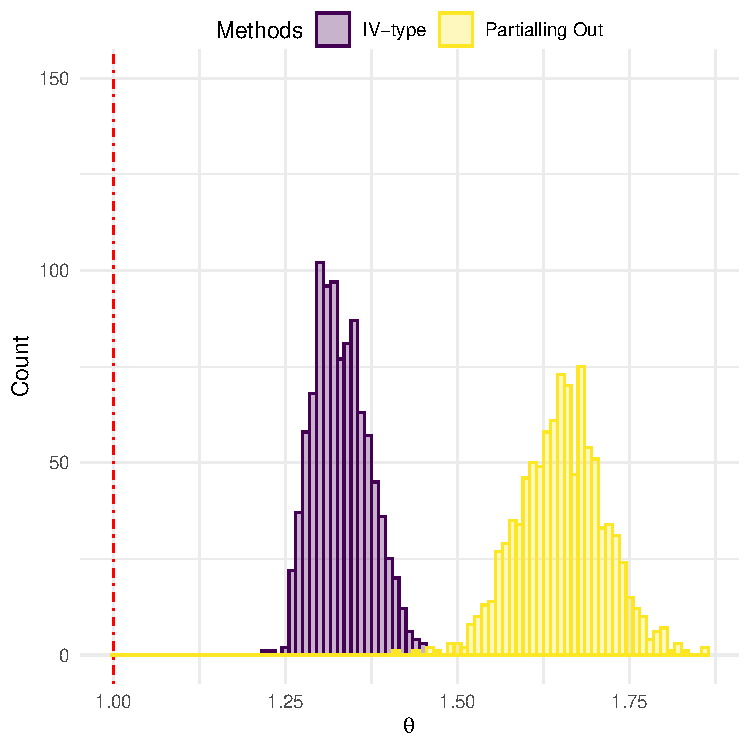
\includegraphics[width=\linewidth]{figures/intution-iv-type-vs-partialling-out-rf.pdf}
        \caption{Random Forest}
    \end{subfigure}
    \caption{}
\end{figure}

\subsection{Complexity of Paramters}

\begin{figure}[htpb]
    \centering
    \begin{subfigure}{.45\textwidth}
        \centering
        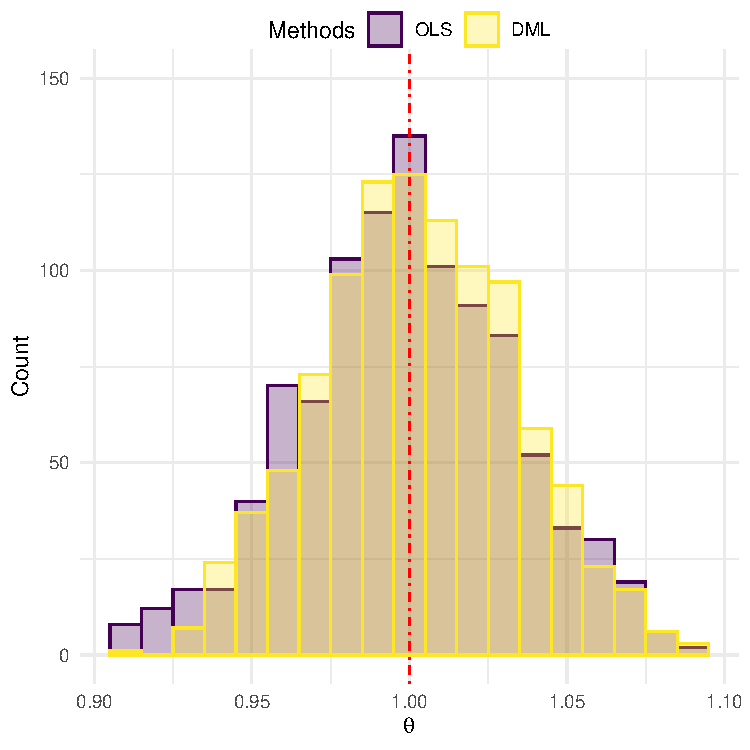
\includegraphics[width=\linewidth]{figures/intution-ols-vs-dml-lasso.pdf}
        \caption{LASSO}
    \end{subfigure}
    \begin{subfigure}{.45\textwidth}
        \centering
        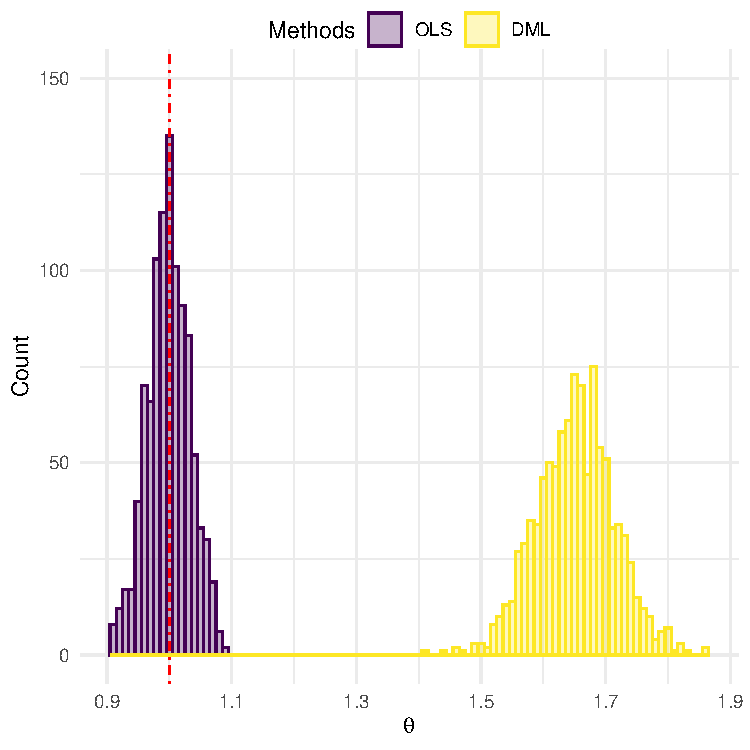
\includegraphics[width=\linewidth]{figures/intution-ols-vs-dml-rf.pdf}
        \caption{Random Forest}
    \end{subfigure}
    \caption{}
\end{figure}

\end{document}